% Bradley Hintze -- Proteins Manuscript
\documentclass[12pt]{article}

\usepackage{authblk}
\usepackage{gensymb,wrapfig,booktabs}
\bibliographystyle{unsrt}
\usepackage[font=small,labelfont=bf]{caption}
\usepackage{fixltx2e}
\usepackage{natbib}
\usepackage{longtable}
\usepackage{graphicx}
\usepackage{subcaption}
\usepackage[bottom=1in, top=1in, left=1in, right=1in]{geometry}
\usepackage{pdflscape}
\usepackage{epstopdf}
\usepackage{url}
\usepackage{amsmath}
\usepackage{setspace}
\usepackage{xcolor}
\usepackage{enumitem}
\graphicspath{{figure_files/}}


%-----------------------------------------------------------------------------%
% HYPERREF: plain black hypertext references for ref's and cite's.
%-----------------------------------------------------------------------------%
\usepackage[pdftex, plainpages=false, 
                                letterpaper, bookmarks, bookmarksnumbered,
                                colorlinks, linkcolor=black, citecolor=black,
                 filecolor=black, urlcolor=black]
                                {hyperref}

\newcommand{\Dmap}{mF$_{o}$-DF$_{c}$}
\newcommand{\EDmap}{2mF$_{o}$-DF$_{c}$}

% These define the color of the changed text in the revision for the editor.
% Choose by commenting out what you DON't want. 
% #FF0000 for red and #000000 for black (i.e. essentially DON'T change color)
%\definecolor{changecolor}{HTML}{000000} %BLACK
\definecolor{changecolor}{HTML}{FF0000} %RED

\begin{document}
\newcommand{\FigOneCaption}{$\chi_1\chi_2$ space for Leu, Ile, and His. The 0.3$\%$ contour outline is in gray. Each point of the background data cloud represents a residue in the filtered Top8000 dataset. Crosshairs mark the nominally ideal staggered values between sp$^{3}$ hybridized atoms, labeled as \textbf{m} (-60$\degree$), \textbf{t} (180$\degree$), and \textbf{p} (+60$\degree$).}

\newcommand{\FigTwoCaption}{Areas in orange (from Top500 data) and in blue (from Top8000) fill the allowed regions for Asp, Trp, and Ile. The extensive areas in green are where the two systems both declare allowed conformations. \textcolor{changecolor}{See Figure S1 for the rest of the two-$\chi$ residues.}}

\newcommand{\FigThreeCaption}{Sidechain contacts for Met A 240 in 2bmo, which adopts the rare methionine rotamer \textbf{ppp}. (a) Sulfur contacts, modeled with ideal staggered dihedrals and Engh \& Huber bond angles, (b) with Engh \& Huber bond angles, but dihedrals as deposited, (c) for the deposited structure, and (d) all contacts for the deposited structure, showing its tight vdW packing.}

\newcommand{\FigFourCaption}{Panel (a) shows the 2.0\% contour surfaces for the filtered Top8000 along with data points, as projected onto the $\chi_{2}$-$\chi_{3}$ plane for rotamers Glu \textbf{pm20} (orange) and \textbf{mp0} (blue). (b) shows how \textbf{pm20} and \textbf{mp0} both make a good H-bond (green dots) with the adjacent backbone NH, albeit through different conformations.}

\newcommand{\FigFiveCaption}{Two different examples of Ile \textbf{pp}, both demonstrating the close C$\delta$1/C contact, and the extensive vdW interactions that prevent the more common \textbf{pt} conformation. (a) 1s99 Ile A 76, (b) 2wvx Ile C 235.}

\newcommand{\FigSixCaption}{3D43 chain B, one of the 11 subtilisins containing a Met \textbf{mpm}. (a) The local arrangement of Ser 250 (red) and Met 251 (blue) on the helix, with the interacting Pro 254 and Ile 246; (b) rotated to show the active site, with its canonical catalytic triad in red and Met 251 in blue.}


\newcommand{\FigSevenCaption}{Filtered Top8000 Asp and Asn datapoints and outlier contours (gray outline). $\chi_2$ does not follow the \textbf{ptm} convention since it is an sp$^{3}$ sp$^{2}$ dihedral.}


\newcommand{\FigEightCaption}{Shown is the $\chi_{1}$ = \textbf{p} slice of the Asn distribution as well as the allowed (green) and outlier (red) contours. Each point in the distribution represents one residue in the filtered dataset. There are several residues that lie outside the outlier contours -- thus are outliers. Two examples that are far from any allowed contour (inside the circle) are shown with excellent \EDmap{} density. These valid outliers both exhibit extensive H-bonding which allows them to be held in an outlier conformation.}


% title page
\title{MolProbity's Ultimate Rotamer-Library Distributions for Model Validation}
\author{Bradley J. Hintze}
\author{Steven M. Lewis}
\author{Jane S. Richardson}
\author{David C. Richardson}
\affil{Department of Biochemistry, Duke University}
\maketitle

\noindent
Short title: MolProbity's Ultimate Rotamer-Library
\newline
\newline
\noindent
Keywords: sidechain rotamer library, rare sidechain conformations, structural bioinformatics, structure validation, Phenix, high-quality dataset, protein conformation
\newline
\newline
\noindent
All work performed at Duke University, Durham, North Carolina.
\newline
\newline
\noindent
Correspondence to: David C. Richardson, 132 Nanaline Duke Building, Duke University, Durham NC 27710. E-mail: dcrjsr@kinemage.biochem.duke.edu


\newpage
\tableofcontents


\begin{doublespacing}

% abstract
\newpage
\section{Abstract}

Here we describe the updated MolProbity rotamer-library distributions derived from an order-of-magnitude larger and more stringently quality-filtered dataset of about 8000 (vs. 500) protein chains, and we explain the resulting changes and improvements to model validation as seen by users. To include only sidechains with satisfactory justification for their given conformation, we added residue-specific filters for electron-density value and model-to-density fit.  The combined new protocol retains a million residues of data, while cleaning up \textcolor{changecolor}{false-positive} noise in the multi-$\chi$ \textcolor{changecolor}{datapoint} distributions.  It enables \textcolor{changecolor}{unambiguous} characterization of conformational clusters nearly 1000-fold less frequent than the most common ones.  We describe examples of local interactions that favor these rare conformations, including the role of authentic covalent bond-angle deviations in enabling presumably strained sidechain conformations. Further, along with \textit{favored} and \textit{outlier}, an \textit{allowed} category (0.3\% to 2.0\% occurrence in reference data) has been added, analogous to Ramachandran validation categories. The new rotamer distributions are used for current rotamer validation in MolProbity and \textit{PHENIX}, and for rotamer choice in \textit{PHENIX} model-building and refinement. The multi-dimensional $\chi$ distributions and Top8000 reference dataset are freely available on GitHub. These rotamers are termed "ultimate" because data sampling and quality are now fully adequate for this task, and also because we believe the future of conformational validation should integrate sidechain and backbone \textcolor{changecolor}{criteria, as opposed to the current independent treatment}.


% text
\newpage
\section{Introduction}
Protein sidechains take on preferred conformations which fall into distinct local energy minima known as rotamers, defined by the set of sidechain dihedral ($\chi$) angles. For tetrahedral geometry, $\chi$ values fall into three discrete ranges: \textbf{p} (plus, centered near +60$\degree$), \textbf{t} (trans, centered near 180$\degree$), and \textbf{m} (minus, centered near -60$\degree$)\textcolor{changecolor}{, as named in\cite{lovell2000penultimate}\footnote{\textcolor{changecolor}{The p, t, m nomenclature was adopted in \cite{lovell2000penultimate} and in MolProbity \cite{Davis2004}, to give a single letter for use in rotamer strings, and because the more common g+, t, g- terminology was, in 2000, still being assigned to opposite conformations (see discussion in \cite{lovell2000penultimate}).}}}. These correspond to low-energy staggered conformations expected between sp$^{3}$ hybridized atoms \cite{Eyring1932}. sp$^{3}$ to sp$^{2}$ bonds (tetrahedral to planar geometries) have more complex and much broader distributions. Overall rotamer conformations, however, are not simply the product of their individual $\chi$ distributions, since wider steric and other atomic interactions influence the preferred, or even the possible, combinations.

Rotamers have been studied extensively since the concept was introduced by Ponder and Richards in 1987 \cite{Ponder1987}, and they are important tools in structural biology \cite{DunbrackJr2002431}. Rotamer libraries classically catalog favored sidechain conformations by the mean $\chi$ values and standard deviations for each rotamer. They are created by performing statistical analysis on a selected dataset of experimentally-determined models, usually crystal structures archived in the Protein Data Bank (PDB) \cite{Berman2000}. Along with Ramachandran backbone $\phi$, $\psi$ analysis \cite{RAMACHANDRAN1963,JSR_theplot_2013}, these libraries form the conformational criteria used in a variety of applications including crystallographic model building and refinement \textcolor{changecolor}{\cite{Arendall2005, Emsley:ba5144, Adams:2010fk, Winn2011, Joosten2011}}, protein structure prediction and design \cite{Bower1997, Kuhlman21112003, Gainza:2012}, and protein model validation \cite{Laskowski:gl0276, Hooft1996, Chen:2010kx}.

Different rotamer libraries represent the allowed variability around each central conformation in one of three ways. Early rotamer libraries simply provided the mean value and some estimate of allowable range for all $\chi$ angles (or, often, just for $\chi$1 and $\chi$2) of each identified rotamer for each side-chain type \cite{Ponder1987, Tuffery1991,Schrauber1993}.  A user would either simply use the mean-value conformation, or else would optimize it manually or computationally within the allowable range. Because modeling the lowest-energy conformation fails to capture allowed variation and further minimization is computationally expensive, design methods expanded to employ "grid" libraries of arbitrarily-spaced, discrete sample points in $\chi$ space around the low-energy mean of each rotamer, which allowed development of the influential Dead-End Elimination method in protein design \cite{DeMaeyer1997,Gainza2013}.  A third type of rotamer software \cite{Dunbrack1997, Chen:2010kx} evaluates a given sidechain conformation by its position in a multi-dimensional probability distribution. Early such distributions were binned (often at $\ge$ 10 $\degree$) \cite{Laskowski:gl0276}, but recent ones use smooth contour surfaces, scored by what percent of the reference data lies outside that contour \cite{lovell2000penultimate, Read2011}. \textcolor{changecolor}{Design libraries and validation libraries focus on two distinct areas of the reference data distributions. While design and prediction are primarily concerned with statistics and cluster shapes inside the low-energy wells \cite{Dunbrack1997}, validation is primarily concerned with robustly identifying the outliers beyond the edges of those wells. Such outliers are usually wrong but sometimes valid and interesting, so are always worth examining \cite{Richardson2013}.}

Because rotamer libraries or distributions are an integral component of modern structural biology, it is imperative that they provide only authentic, low-energy sidechain conformations so that errors are not propagated. Such errors of circular reasoning can be documented \cite{lovell2000penultimate} for many early cases, such as high-energy eclipsed $\chi$ angles added for "completeness", or real empirical data clusters caused by incorrect backward-fit branched sidechains. The accuracy of these libraries depends on including only reliably modeled sidechains in the reference dataset. All rotamer libraries filter their datasets at the file level by resolution and redundancy. As the PDB grew in size, it  became increasingly practical to filter also at the residue level. This process very effectively lowers noise and sharpens clustering, because even at high resolution the poorly ordered regions are susceptible to misfitting and are often worse than the good parts at low resolution.

Previously our group developed the "penultimate" rotamer library, using the quality-filtered Top240 PDBs \cite{lovell2000penultimate}. Soon afterward we updated the library using our Top500 dataset \cite{Lovell:2003uq}. This library used many file-level filters such as requiring $\le$ 1.8 resolution, a clashscore $<$ 30 \cite{Word1999}, and few backbone bond-angle outliers from Engh and Huber standards \cite{Engh1991}, \textcolor{changecolor}{and when the file contained multiple identical chains, used only the best-ordered one}. The residue-level filters required a B factor $<$ 40 for all atoms in the residue and the absence of serious steric clashes, defined as hydrogen-aware atomic overlaps $\ge$ 0.4 \AA \cite{Word1999}. These filters were used in order to eliminate residues with questionable justification for their given conformation, thereby increasing reliability. Specifically, the B-factor filter (the best metric available before mandatory data deposition) was meant to eliminate residues with poor electron density or other local uncertainty. However, as we realized and as Shapovalov and Dunbrack later clearly demonstrated \cite{Shapovalov:2007}, in many structures the B factors are a poor indicator of good density, primarily because they are often restrained to change only modestly between adjacent, covalently bonded atoms. Since 2008, when the wwPDB started requiring structure-factor data with all depositions, it has become feasible to do routine analysis of electron density directly.

In the current work we use a new quality-filtered dataset curated by our lab, the Top8000, to develop a new rotamer library. The main differences between this dataset and our previous dataset are sheer size (8000 vs. 500 chains) and improved quality filters, which are stricter and better balanced at the \textcolor{changecolor}{overall file (or chain)} level and especially at the residue level. We now use a three-component residue filter that adds real-space correlation coefficient (RSCC) and local map value to B factor, effectively eliminating all residues with poor electron density. We explain how these strict filters reveal authentic, rare, and interesting rotameric states, including cases where bond angles must open up significantly. The improved statistics enable a three-level rotamer classification for validation of \textit{favored}, \textit{allowed}, and \textit{outlier} (analogous to classic Ramachandran measures), where now only 0.3\%, rather than the previous 1.0\%, of the high-quality, filtered reference data lies outside both the \textit{allowed} and the \textit{favored} regions.

\section{Methods}
\subsection{Chain-level Dataset Filters}
Our previous rotamer library \cite{lovell2000penultimate} used the Top500 quality-filtered data \citep{Lovell:2003uq} as its reference dataset. Since then the number of high-resolution structures in the PDB has skyrocketed, allowing us to create a new quality-filtered, X-ray model database, the Top8000. The Top8000 was curated by assessing all PDB crystal structures as of March 29, 2011 with a protein chain of $\ge$ 38 residues at $<$ 2.0 \AA{} resolution. Hydrogens were added to each PDB file using Reduce, including Asn, Gln, and His flip corrections \citep{Word19991735}. MolProbity analysis was performed on each chain \citep{Chen:2010kx} and the results entered into a MySQL database. The chains were additionally filtered on the following criteria: chain MolProbity score $<$ 2.0, $\le$ 5\% of residues with bond length outliers ($>$ 4$\sigma$), $\le$ 5\% of residues with bond angle outliers ($>$ 4$\sigma$), and $\le$ 5\% of residues with C$\beta$ deviation outliers ($>$ 0.25\AA{}).

In order to control redundancy in the dataset, we made use of the PDB homology clusters, taken separately for 50\% sequence identity (most stringent similarity filtering), 70\%, 90\%, and 95\%. For each homology cluster, we selected the best chain based on the average of resolution and chain MolProbity score. This scoring scheme produced ties within some clusters (for $<$ 1\% of the final chain tallies); these were resolved, arbitrarily but reproducibly, by alphabetical order of PDB ID + single-character chain ID. At each homology level, a second list was chosen with the additional requirement of deposited structure-factor data. All 8 chain lists are available on GitHub \citep{Dabbish:2012} (e.g. file \texttt{Top8000-SFbest\_hom70\_pdb\_chain\_list.csv}, at \url{http://github.com/rlabduke/reference_data}). The "SF" lists are somewhat smaller, since some clusters may include no otherwise-acceptable structures with deposited data. At the 70\% similarity level optimal for most data-mining purposes, the Top8000-SFbest\_hom70 list contains 7,419 chains and the Top8000-best\_hom70 list contains 7,957 chains. This entire set of datasets is therefore nicknamed the "Top8000" of structural biology's upper class.

All rotamer statistical analysis presented here used the Top8000-SFbest\_hom70 dataset version. Deposited structure factors not only are required for electron-density based residue filtering, but they also enable examination of the model in the density map for individual examples of conformations deemed dubious or interesting. Of the 7,419 chains, 28 failed in the RSCC calculation described below, and 175 were dropped because $\le$ 20\% of their residues remained after residue-level filtering. The final rotamer dataset of 7,216 chains is listed in the supplementary material.


\subsection{Residue-level Dataset Filters}
\label{sec:resfilters}
Although the chain-level filters select for structures with high overall quality, local quality varies considerably within any model. In this context, \emph{quality} refers to canonical macromolecular model validation criteria (sterics, geometry, and conformation) as well as the fit to electron density. An important aspect of this research is to include only amino-acid sidechains with sufficiently clear electron density to justify their given conformation. Our previous rotamer library was based on the Top500 dataset where only two residue-level filters were used: no clashes and no B factors $\ge$ 40 \AA\textsuperscript{2}. The B factor filter was then (in 2003) our best available proxy for electron-density quality; however, residues with dubious sidechain density still remained. To remedy this, the current dataset was also filtered by a local real-space correlation coefficient (RSCC) metric and by local map value.

\begin{equation}
RSCC = \frac{\sum_{i=1}^{n} \left ( o_{i} - \bar{o} \right )\left ( c_{i} - \bar{c} \right )}{\sqrt{\sum_{i=1}^{n} \left ( o_{i} - \bar{o} \right )^{2} \ast \sum_{i=1}^{n}\left ( c_{i} - \bar{c} \right )^{2}}}
\label{rscceq}
\end{equation}

The local RSCC looks at the correlation between the $\sigma_{A}$-weighted \EDmap{} and the F$_{c}$ (calculated from model) electron density maps for a given local region, in this case, around each individual atom. Equation \ref{rscceq} shows how the RSCC was calculated. $o$ and $c$ are $\sigma$ values at grid points in the \EDmap{} and the F$_{c}$ maps, respectively, in a radius around the atom. The radius used is resolution dependent; a 1\AA{} radius is used for resolutions below 1\AA{} and a 1.5\AA{} radius is used for resolutions between 1\AA{} and 2\AA{}. $n$ is the number of grid points in the selected region and $\bar{o}$ and $\bar{c}$ are the local mean values for $o$ and $c$, respectively. The RSCC alone is not an adequate density-fit metric for our purposes. However, local RSCC (for shape), local \EDmap{} $\sigma$ value at the atom coordinate (for height), and B factor (for spread) together create a satisfactory fit-to-density metric. We used \textit{phenix.real\_space\_correlation} in the \textit{PHENIX} software package \citep{Adams:2010fk} to calculate the RSCC and \EDmap{} $\sigma$ values at each atom for all structures in the Top8000. Per-residue filter values were then assigned by taking the worst atom B (greatest value), worst atom RSCC (least value), and worst atom \EDmap{} $\sigma$ value (least value) in each residue.

In selecting filter thresholds for the dataset, we had the goal of keeping a large number of residues while reliably eliminating those with dubious density. To do this, we analyzed the counts of residues remaining for several combinations of filter thresholds. The best balance between filter levels and a reasonably large number of residues yielded the following thresholds: worst B factor $<$ 40, worst correlation coefficient $>$ 0.7, and worst map value $>$ 1.1. Upon visual inspection of residues and maps close to these filter thresholds, we determined that the selected combination of thresholds was indeed effective at keeping only residues with satisfactory electron density. Additionally, residues were required to have no all-atom clashes, an occupancy of 1.0, B factors $>$ 1.0 and all backbone atoms modeled, achieved indirectly by ensuring that $\phi$, $\psi$, $\omega$ and $\tau$ were defined for each residue.  The latter test also drops sidechains of the first and last residue in each chain, which are somewhat less and differently affected by backbone interactions.

After all filters, the final reference dataset for this work contains more than a million residues, 983,574 of which are rotamer-relevant, non-Gly non-Ala residues. A csv file of all 983,574 residues in the rotamer-relevant reference dataset is available on GitHub (See \texttt{datasets/Top8000\_rotamer\_residues.csv} at \url{http://github.com/rlabduke/reference_data}).

\subsection{Determination of Distributions, Scores, and Contours}
\label{sec_md:contours}
The described rotamer library's primary use is for validation of sidechains in protein models, which flags an outlier if the sidechain has an extremely rare (and presumably high-energy) conformation. This assessment requires a scoring system based upon the multi-dimensional distribution of observed conformations in our high-quality, residue-filtered reference data. We have taken great care to ensure smooth, accurate, and robust contours dividing outlier from allowed. To achieve this we calculated smooth distributions in the multi-dimensional $\chi$ space for each residue type, using an adaptive local-density-dependent kernel density estimation (KDE). Our method has two steps, both using a cosine kernel normalized to have an area or volume of 1.0. A cosine is used, rather than a gaussian, because it reaches zero at a well-defined edge. In the first step, the width of each cosine kernel is 5$^{\circ}$. In the second step, the width of the kernel is varied, dependent on the density at that location, as calculated in the first step. Kernel widths are wider in sparse regions and narrower as density increases. The consequence of this is distributions that remain smooth in sparse regions but preserve the sharp transitions where occurrence frequency falls off quickly. A full explanation of this method can be found in \cite{Lovell:2003uq}. The distributions are stored as a discrete grid in $\chi$ space with coordinates and KDE values. Grid spacing is dependent on dimension number: in order of $\chi$ dimensions, 1-4, the grid spacings are 1, 5, 8, and 10 degrees. Each datapoint residue can be assigned a value by interpolating its $\chi$ values within the grid. One can then determine what grid value is just greater than for the lowest, say, 1\% of the quality-filtered reference data. The grid values are then rescaled to represent those percentage values, which are known as the \textit{rotamericity} of a sidechain conformation, or simply as the rotamer score. The rotamer-score grids are used in \textit{PHENIX} validation (GUI, \texttt{phenix.rotalyze}, and \texttt{phenix.molprobity}) and the MolProbity web service, and they are available as plain-text numerical arrays on GitHub, under \texttt{datasets/Top8000\_rotamer\_pct\_contour\_grids} at \url{http://github.com/rlabduke/reference_data}.

To visualize the rotamer distributions, smooth contours are drawn at chosen levels using our internal programs Silk, kin2Dcont, and kin3Dcont \cite{Thesis:Word,Thesis:Davis}. For the 4-dimensional Lys and Arg cases, the 3-D plots for $\chi$1\textbf{m}, $\chi$1\textbf{t}, and $\chi$1\textbf{p} are shown separately. For validation purposes, the interpolated grid value of a given multi-$\chi$ conformation is its rotamer score. In the new system developed here, a score of $\le$0.3\% qualifies as a rotamer outlier -- its score is worse than 99.7\% of the good data. Scores $>$0.3\% and $<$ 2.0\% are considered \textit{allowed} while those $\ge$2.0\% are considered \textit{favored}, as is traditional for Ramachandran criteria \citep{Laskowski:gl0276,Lovell:2003uq}.

\subsection{$\chi$ and Covalent Bond Angle Statistics}
\label{sec_md:chi_stats}
Maximum rotamer ranges were defined manually for each $\chi$ dimension by inspecting the smoothed contours (See \ref{sec_md:contours}) and placing boundaries at saddle points between rotamers or to reasonably encompass the rotamer well. To avoid wrapping complications, circular statistics were used (See Equations \ref{circ_xy} and \ref{circ_s}); this is important for $\chi$ distributions that cross zero, such as Asp \textbf{p0} and \textbf{m-30}, or for rotamers near 90$^{\circ}$ in symmetric aromatics. For each rotamer, we report a central value and a standard deviation ($\sigma$), for both dihedral $\chi$ values and covalent bond angles. The mean for the bond angles (Equation \ref{circ_m}) and the $\sigma$ for both $\chi$ and bond angles (Equation \ref{circ_s}) are calculated straightforwardly from the measures of each example in the filtered Top8000. Because of complex shapes, the central value for the $\chi$ measures is the center-of-mass (COM) in the contoured data. This is found by collecting the stored contour grid points in each rotamer well and, for each dimension, calculating the COM (Equation \ref{circ_com}).

\begin{equation}
\bar{x} = \frac{\sum_{i=1}^{n}\left ( \sin \theta_{i} \right )}{n}
\textrm{, }
\bar{y} = \frac{\sum_{i=1}^{n}\left ( \cos \theta_{i} \right )}{n}
\label{circ_xy}
\end{equation}

\begin{equation}
\sigma = \sqrt{-2 \ln \left ( \sqrt{\bar{x}^{2} + \bar{y}^{2}} \right )}
\label{circ_s}
\end{equation}

\begin{equation}
\textrm{mean} = \arctan\left (
\frac{\bar{x}}{\bar{y}}
\right )
\label{circ_m}
\end{equation}

\begin{equation}
\textrm{COM} = \arctan\left (
  \dfrac{
    \dfrac{\sum_{i=1}^{n}\left ( \sin \theta_{i} \right )\ast w_{i}}{W}
  }{
    \dfrac{\sum_{i=1}^{n} \left ( \cos \theta_{i} \right )\ast w_{i}}{W}
  }
\right )
\label{circ_com}
\end{equation}

\noindent where $n$ is the number of grid points, $\theta_{i}$ is the $i^{th}$ $\chi$ coordinate in radians, $w_{i}$ is the KDE value at the $i^{th}$ coordinate and $W$ is the sum of all KDE values in the rotamer well. To avoid wrapping issues when working with angular data, circular statistics breaks angle measures into its two unit circle components, $x$ and $y$. This is part of what is being done in Equation \ref{circ_xy}, where $\bar{x}$ and $\bar{y}$ are the average $x$ and $y$ components, respectively, for all angular measures, $\theta$. In Equation \ref{circ_com}, a weighted average of the $x$ and $y$ components is being calculated. The arctan function simply takes the $\bar{x}$ and $\bar{y}$ components and returns the corresponding angular value.

\subsection{Rotamer Assignment and Score}
\label{sec_md:rotaassign}
For the purpose of setting the appropriate contour level for the outlier cutoff, a large test dataset was created from all PDBs in the Top8000 by including all chains and all residues in each PDB file (as a surrogate for entire new PDB files later being validated), hereafter called the unfiltered dataset. \textit{phenix.rotalyze} was used to assign rotamer names and scores for each residue in the unfiltered dataset. The score is calculated from the individual residue's $\chi$ values, by interpolating over the nearest contour grid points (see section \ref{sec_md:contours}). This was done twice, once using the new Top8000 contours and once using our previous Top500 contours. If the score is above the outlier threshold, then a rotamer name is assigned based on which rotamer well the given $\chi$ angles fall within (the maximum well ranges were described in Section \ref{sec_md:chi_stats}). Otherwise the side-chain conformation is classified as an \textit{outlier}.
\section{Results}
In the Top8000 system there are a total of 234 named rotamers which reach above the 0.3\% outlier cutoff and \textcolor{changecolor}{which passed manual examination of all examples within clusters that include $\le$ 8 datapoints (only two such clusters failed the test: both were Lys rotamers with $\le$ 4 datapoints)}. Many of the central values have shifted somewhat from the Top500 system, both because of much more and higher-quality data and also because of the new center-of-mass definition (see Section \ref{sec_md:chi_stats}), which we feel represents the clusters better than either the modal or the common-atom values defined previously \cite{lovell2000penultimate}. MolProbity's "ultimate" rotamers and their parameters are given in two tables: Table S3 describes the frequency and count of each rotamer in each residue type and Tables S4-S21 give central dihedral and covalent angle values for each rotamer. These numbers are available in CSV format on GitHub under \texttt{Top8000/Top8000\_rotamer\_central\_values} at \url{http://github.com/rlabduke/reference_data}. The more useful multi-dimensional distributions are also on GitHub, as linked in Section \ref{sec_md:contours}.

The order-of-magnitude increase in size and quality of our reference dataset greatly improves signal-to-noise, allowing us to do a better job of the same functions as before. More importantly, it enables new features and new conclusions. The simplest view of a rotamer is of a favored sidechain conformation described by the list of dihedral angles, with ideal staggered $\chi$ values between sp$^{3}$ atoms and little preference for $\chi$ between sp$^{3}$ and sp$^{2}$ atoms. The next level of detail adds a standard deviation for each $\chi$. However, conformational preferences are really much more complex, especially in a macromolecular interior where numerous interactions can compensate for the energy required to depart from ideal. We have high confidence in the reliability of our more nuanced conformational distributions, as we took great care to include only physically plausible sidechains that fit clear electron density (see Section \ref{sec:resfilters}). As Figure \ref{fig:outcontour} demonstrates, sidechain conformations do cluster in discrete regions of $\chi$ space. Further, there is large variance in $\chi$ values within a rotamer cluster, the shape is usually not axis-oriented, and its center is rarely at the nominally ideal staggered conformation. A rotamer is better thought of as a local energy well, with a potentially complex shape, describing the favorable extent around an allowed sidechain conformation.

\subsection{Residue Filter Effects}
\label{sec_rs:filterdataset}
Our strict residue-level filtering aims to include essentially only conformations with unassailable reliability, at some expense to the overall numbers. The fraction of  residues kept after filtering differed between amino-acid types (Table S1). Residue-level filtering eliminated the most data, in order, for lysine, glutamate, and arginine. This makes sense since long sidechains are more susceptible to dynamics that can blur or eliminate density. Also, charged sidechains are usually found on the molecular surface interacting with mobile solvent. Hence, surface-exposed positions such as these, lacking strong interactions that can hold them in a disfavored conformation, have no need and no ability to adopt rare, unfavored rotamers. If such sidechains are modeled, they should be in one, or more often several, common rotamers.

\subsection{Rotamer Evaluation}
\label{sec_rs:rotaeval}
The primary purpose of this rotamer library is to analyze the rotamericity of protein sidechain conformations and robustly distinguish outliers. Rotamericity here refers to where a given conformation lies in $\chi$ space relative to the calculated contours (see Section \ref{sec_md:contours}). This evaluation gives a rotamer score between 0 and 100, corresponding to the percentage of the high-quality reference data that lies outside that contour (i.e., how much of the reference data's scores are worse than the given residue). In addition, for scores above the outlier cutoff, the evaluation also assigns a rotamer name. Each local minimum, or cluster, in $\chi$ space is given a name derived from the central $\chi$ values of that cluster. Values for $\chi$s between sp$^{3}$ hybridized atoms are named \textbf{m}, \textbf{p}, or \textbf{t} roughly corresponding to the staggered values -60$\degree$, +60$\degree$ and 180$\degree$. $\chi$s between sp$^{3}$ and sp$^{2}$ hybridized atoms are assigned a number which is the COM value (Section \ref{sec_md:chi_stats}) of the given $\chi$, rounded off. For instance, a Gln rotamer with COM at $\chi_1$ = -174, $\chi_2$ = -82, and $\chi_3$ = -22 is named \textbf{tm}-20.

For validation purposes, users are often most interested in the binary issue of whether a sidechain conformation is rotameric or an outlier, i.e. falls within or outside the rotamer distribution. With the Top500 data, contours were smooth and reproducible (between different datapoint selections) only out to the 1\% level. Due to greater numbers and increased reliability in the filtered Top8000 distributions, a lower outlier cutoff is now feasible as well as desirable, since an even lower percentage of the reference datapoints are now dubious. We also preferred to keep outlier numbers for unfiltered, general data roughly equal between the previous and new systems. Therefore a count of the 1\% outliers by residue type in the unfiltered dataset was performed using the Top500 contours, and those numbers were compared to outlier counts at several different Top8000 contour cutoffs. A new cutoff of 0.3\% matched best, was found to behave smoothly, and happens also to match the 3$\sigma$ level for a normal distribution (3 out of 1000). \textcolor{changecolor}{Table S2 reports the outlier counts in the unfiltered dataset for both the Top500 and Top8000 contours.} Further, along with favored and outlier, a new category has now been added: \textit{allowed}, for scores $\ge$0.3\% and $<$2.0\%. This new category lets users know if a given conformation is at the edge of the given rotamer's distribution, close to the outlier region. This change matches the 3-part system, and the division at 2.0\%, long judged useful for Ramachandran criteria \cite{Kleywegt1996, Hooft1996, Lovell:2003uq}.

An important question is how the new system will change rotamer analysis, specifically the number and identity of outliers. A rotamer outlier is simply a conformation that lies outside the outlier contours of the reference dataset, in this case either the Top500 or the Top8000. For residues that have low-energy sidechain conformations, nothing will change. However, a sidechain conformer in a strained position near the outlier edge could change status between the Top500 and Top8000 analyses. Figure\textcolor{changecolor}{s} \ref{fig:contour_compare} \textcolor{changecolor}{and S1 show} Top500 and Top8000 allowed regions superimposed for \textcolor{changecolor}{all residues with two $\chi$s}. For the most part, the contours overlap, but with some differences near the edges. Asp shows very little change, Trp has a significantly larger allowed region now than in the Top500 system, and the Ile Top8000 contours have tightened up relative to the Top500. Thus, differences are only in low-population regions of $\chi$ space, and overall outlier counts will be nearly identical.

\subsection{Dihedral and Bond Angle Deviations}
As we have shown, rotamers are more complex than just a collection of mean $\chi$ values and standard deviations. The allowed regions are often large and complex, and the mean or modal $\chi$ angles can \textcolor{changecolor}{deviate substantially from the expected staggered conformation}. Such deviations usually occur in well-packed environments where the sidechain makes \textcolor{changecolor}{tight atom-atom} interactions, either via van der Waals (vdW) or H-bonding, with its own backbone (or within the sidechain). The $\chi$ deviations help allow the contact to be \textcolor{changecolor}{a small overlap} rather than a steric clash.

For sidechains that have sp$^{3}$ atoms out to the $\delta$ atom (Leu, Ile, Met, Glu, Gln, and Arg), there are four $\chi_{1}\chi_{2}$ combinations that produce close sidechain-backbone interactions; \textbf{pm} and \textbf{mp} interact with the NH while \textbf{tm} and \textbf{pp} interact with the carbonyl C. Comparing statistics on all $\chi_{1}\chi_{2}$ combinations for these amino acids in the filtered dataset (Table \ref{tab:chi12}), we see that the backbone-interacting combinations are the least populated and that they have large $\chi$ deviations from the ideal staggered positions, especially for $\chi_{2}$. 

Breaking down these statistics by residue type reveals that Glu and Gln make up 54.3\% of \textbf{mp}, 59.8\% of \textbf{tm}, and 92.2\% of \textbf{pm} examples. The likely reason for this is that the terminal oxygens on Glu and Gln can H-bond with their own NH for \textbf{pm} and \textbf{mp}. In \textbf{tm} a strong vdW interaction is made with the C-terminal peptide plane, and the sidechain amide or carboxyl group is generally further stabilized by one, or more often multiple, H-bonds. However, as for all sidechain-backbone interacting rotamers, the dihedral $\chi$ deviations don't tell the whole story -- covalent bond angles also must deviate to avoid steric clashes.

It has long been known that certain sidechain conformations show large deviations in the otherwise narrowly distributed covalent bond angles \cite{lovell2000penultimate}; this is seen in the scenarios above where sidechain-backbone interactions occur. One rotamer of this type is methionine \textbf{ppp}, which has just 48 examples (0.29\% of Met) in the filtered Top8000. Figure \ref{fig:2bmo} shows one specific example and demonstrates how deviations in \textit{both} $\chi$ dihedrals and covalent bond angles are needed to avoid a clash and form a favorable non-bonded interaction. All-atom contacts demonstrate the tight vdW packing. For this residue, the angles C-C$\alpha$-C$\beta$, C$\alpha$-C$\beta$-C$\gamma$, and C$\beta$-C$\gamma$-S$\delta$ each open up from Engh \& Huber values, by +1.6$\degree$, +0.9$\degree$, and +3.0$\degree$ respectively.

\subsection{Interesting Rotamer Anecdotes}
Consistently large deviations from ideal values in the $\chi$ and covalent bond angles for some rotamers raise two questions, which are interesting and sometimes illuminating: (1) What is it about each of these rotamers that requires such deviations? (2) What are the structural features and roles for each of these rotamers? These questions were answered by inspecting individual examples from the filtered dataset. After an interesting rotamer was identified, at least five random examples of that rotamer were selected from the filtered dataset. To visualize interactions for the residue of interest, all-atom contacts were displayed in KiNG \cite{Chen2009}. This process revealed commonalities of the rotamer environment, reasons for the deviations, and possible reasons for a rare rotamer frequency. What follows are select observations from this process.

\subsubsection{Glutamate \textbf{pm20} \& \textbf{mp0}}
Glutamate \textbf{pm20} and \textbf{mp0} make up 2.6\% and 6.4\% of all glutamates in our dataset and would not be considered rare in the context of this paper. These rotamers are of interest, however, for three reasons: (1) some average $\chi$ and bond angles have relatively large deviations from ideal (Table \ref{glupangles}), (2) despite this, these rotamers are significantly more common than other rotamers with similar deviations, and (3) the $\chi$ distributions for both show that all three $\chi$ measures strongly depend on one another, forming correlated datapoint clusters (Figure \ref{fig:Glupm20_mp0}a). In both \textbf{pm20} and \textbf{mp0}, the same carboxylate oxygen makes a strong H-bond with its own NH, but they take a different path to do so (Figure \ref{fig:Glupm20_mp0}b). The large geometry deviations are required in order to avoid a steric clash of C$\delta$ with the backbone.  Glutamine can adopt equivalent arrangements, as previously noted even from much sparser data \cite{Lovell1999}.

The strong sidechain-backbone H-bond, between atoms separated by only 5 covalent bonds, is an important characteristic of these conformations.  It compensates for the energetic cost of distortions better than would a vdW contact, and especially it gives rise to a characteristic interdependence of the three $\chi$ angles: as one $\chi$ changes, the others change in predictably compensating ways to preserve the favorable H-bond.


\subsubsection{Isoleucine \textbf{pp}}
With just 249 examples in the filtered Top8000, \textbf{pp} is the rarest isoleucine rotamer. This rotamer epitomizes most rare ones, by having numerous surrounding vdW interactions to pack the sidechain into this specific rotamer state, which is rare because of strain from its need for large average bond and dihedral angle distortions. The modal $\chi_{2}$ value is +24.3$\degree$ from staggered and bond angles C$\alpha$-C$\beta$-C$\gamma$1 and C$\beta$-C$\gamma$1-C$\delta$1 open, relative to Engh \& Huber, by 2$\degree$ and 1$\degree$, respectively (Table \ref{tab:ilepp}). In \textbf{pp} the terminal methyl is in the "down" position approximately parallel to the course of the backbone (Figure \ref{fig:Ilepp}). In all examples examined, local structure packed the methyl into this rare conformation by sterically prohibiting the more common \textbf{pt} rotamer (methyl "up"). The resulting bond-angle and dihedral openings are necessary to minimize a steric clash between C$\delta$1 and the backbone C.

\subsubsection{Methionine \textbf{mpm}}
Methionine \textbf{mpm} is extremely rare, with only 13 examples in the filtered Top8000. The deviations from ideal are remarkable: C$\alpha$-C$\beta$-C$\gamma$ and C$\beta$-C$\gamma$-S$\delta$ open by more than 2$^\circ$ and 3$^\circ$, respectively, and the modal $\chi_{3}$ in \textbf{mpm} is a mere 20$^{\circ}$ from being eclipsed -- probably permitted by the fact that $\chi_{3}$ in Met has a lower rotational barrier than all-carbon tetrahedral torsions because of the longer C-S bond \cite{Butterfoss2003, Butterfoss2004}. Here, if $\chi_{3}$ were any closer to staggered, the $\epsilon$-methyl would clash with its backbone NH. 

Out of the 13 Met \textbf{mpm} examples in the filtered Top8000, 11 are structurally very similar, with much of the surrounding sequence identical. All 11 belong to the large superfamily of subtilisin-like serine proteases, which contains six families A-F. A large multi-sequence alignment (\cite{Siezen1997}) reveals that the Met is completely conserved in families A, B, and C, absent in D and E, and mostly present in F. The Met occurs in the first turn of a helix that is disrupted n+3 to the Met by a proline conserved in the same families (Figure \ref{fig:METmpm_3d43}a). Most significantly, immediately preceding the Met is the Ser of the canonical Asp-His-Ser catalytic triad (Figure \ref{fig:METmpm_3d43}b). Figure \ref{fig:METmpm_3d43}a shows the extensive contact between the catalytic Ser and the \textbf{mpm} Met. Also shown is the extensive contact between the Met and Ile 246, which excludes the possibility of Met $\chi_{3}$ adopting either a \textbf{p} or \textbf{t} conformation. Although the identity of residue 246 changes across the 11 structures, the constraining hydrophobic contact is maintained. 

This case illustrates that 70\% homology filtering does not always produce independent examples when a rotamer is conserved for functional reasons. In the families where the Met is conserved, it seems structurally important as part of a motif packing tightly with the catalytic Ser.  However, in families where the Met is missing, no other sidechain fills in to sterically position the active Ser.  Therefore the functional reason for conservation must be more subtle, at the frontier of our understanding.  Experimental research will be needed to untangle its effects on catalysis.

\subsection{Conformations Between Tetrahedral and Planar Atoms}
Due to differing physical constraints, dihedral angles between tetrahedral and planar atoms do not follow the well-clustered \textbf{ptm} conformations seen between two tetrahedral atoms: when one planar sp$^{2}$ branch is staggered the other is eclipsed. This is reflected in the Top8000 filtered distributions where sp$^{3}$-sp$^{2}$ dihedrals  (always in the final $\chi$ of the sidechain) often show only weak preferences across their total range (e.g., see Figure \ref{fig:outcontour} for $\chi_{2}$ of histidine).

For the aspartate and asparagine contours shown in Figure \ref{fig:AspAsn}, sometimes $\chi_{2}$ has disallowed regions and sometimes the entire range is allowed. This fact makes it even more difficult, and less meaningful, to assign a central value and standard deviation that adequately describes the allowed conformations. Asp and Asn also show clearly that there is distinct, complex fine-structure of local clustering in the data distributions; \textcolor{changecolor}{note especially the smaller elongated clusters at top right of $\chi_{1}$ \textbf{t}}. These datapoint clusters are primarily due to patterns of sidechain H-bonding to specific backbone donors or acceptors local in sequence, or occasionally due to especially favorable vdW packing against local backbone.  For example, the Asn N$\delta$2 can either H-bond with the i-4 CO in a regular $\alpha$-helix in an \textbf{m-80} conformer or pack against that CO in the more common \textbf{m-20} conformer \cite{Lovell1999}.

Both these issues confirm that a complex probability density function, such as our filtered and smoothed empirical contours, represents sidechain conformational preferences much better than a library of simple box or ellipsoid shapes. Its contour outline at low probability is a definitive way to flag rotamer outliers.  For protein structure prediction or design, the details of favored local motifs at high contour levels should also be considered, preferably with the addition of information both about $\phi$,$\psi$ values \cite{Bower1997} and local secondary structure \cite{lovell2000penultimate}. \textcolor{changecolor}{Either as a library or as a distribution, it is preferable to avoid the "rare" rotamers (identified in Table S3) unless the other data is robust enough to support assignment of a very low-probability conformation.}

\section{Discussion}

\subsection{In what sense is this ultimate?}
Calling this set of rotamer-library distributions "ultimate" is a claim that requires both explanation and justification. 16 years after our "penultimate" rotamers, we had to confront the issue of whether or not MolProbity's line of validation-focused rotamer distributions had reached its ultimate stage. We decided that indeed it had, from three separate line of arguments.

(1) We claim it as ultimate for validation (where outlier status is pre-eminent)  -- such as done by the MolProbity website, in \textit{PHENIX}, or by the wwPDB. We are not advocating for this to be an "ultimate" library for other purposes (such as protein design and prediction) which depend on accurate comparisons within the regions of high probability rather than on accurate delineation of the outer limits of those regions.

(2) The quantitative changes from the penultimate distributions are fairly minor. The important new feature is the ability to support a 3-level evaluation to identify very rare rotamers and to specify rotamer-dependent bond-angle deviations. The task of robustly locating contours that separate favored (98\%), allowed, and outlier regions are made possible due to the large number (a million) of reliably-modeled residues. The results are thus unlikely to change much in the future, except for some special cases not examined here such as disulfides and chemically modified amino acids.

(3) The inevitable expansion of data and compute power, as well as needs of structure determination at lower resolution, will change how sidechain modeling and validation is defined. Rather than separate Ramachandran and rotamer evaluation, we should move toward analyzing all backbone and sidechain torsional dimensions together \cite{JSR_theplot_2013}, including allowance for the influence of secondary structure and local motifs. Thus our "ultimate" claim asserts the position that MolProbity's type of rotamer evaluation should no longer be updated but should evolve into something better.

\subsection{Use of the Top8000 rotamer distributions in model building}
Although the Top8000 rotamer distributions were created specifically for MolProbity's validation of sidechain conformations, they also can be used in model building for crystallography, design, homology, etc., as the Top500 library has been \cite{Langer2008, Emsley:ba5144, Headd2008, Terwilliger2008, Adams:2010fk, Gainza2013}. To make model building computationally tractable, sidechains are initially fit as discrete conformations at rotamer values, then either minimized or tested at neighboring sample points using $\sigma$ to inform the allowable range for each $\chi$. However, most rotamer distributions are far from normal and often have quite complex shapes, as can be seen in Figures \ref{fig:AspAsn} and \ref{fig:outcontour}. Thus the approach of using a central value and $\sigma$ cannot adequately describe allowed sidechain conformations. 

The contour values in our rotamer distributions correspond to the percentage of high-quality reference data that lies outside that contour. The consequence of this treatment is that the contour data represent a probability density function in $\chi$ space describing sidechain conformations. We recommend using those contours to delimit sampling or minimization in $\chi$ space, with the added benefit that the contour levels provide prior probabilities for each position. If a contour level higher than 0.3\% is chosen for this purpose, then rotamers which do not reach the chosen percentage level should be omitted. Depending on details of the algorithm used, it may or may not be beneficial to model significant rotamer-dependent bond-angle deviations.

\subsection{I have a rotamer outlier; is it wrong?}
An accurate macromolecular model gives unparalleled mechanistic knowledge at the single-molecule level. Many such models, of different cellular components, combined with structural perturbations such as point mutations and ligand binding, provide mechanistic detail on the cellular level. These methods not only provide interesting knowledge, they allow understanding crucial to the treatment of disease. The utility of a model in this process is correlated with how accurate it is. As such, structural biologists want to build models that come as close as possible to representing a valid state of the actual macromolecule. Unfortunately, the experimental data alone seldom provide all information needed to build an adequate model. Fortunately, empirical knowledge of chemical and macromolecular structure helps greatly, and in crystallography much of this knowledge (e.g. bond lengths and angles, chirality) is already part of the automated software. Structure validation such as MolProbity provides even more empirical knowledge, often highlighting errors that refinement was unable to fix.

Sometimes we get disturbing reports that people are trying to achieve a sort of "MolProbity Nirvana" by attempting to eliminate every single outlier. To approach eliminating all clashes is a worthy goal: in principle the clash target is zero, as sterics do not allow serious atomic overlaps. However, at high resolution a zero score would require the difficult reconciliation of occupancies for alternate conformations including waters, and in any case a few puzzles often remain. Another important point to keep in mind is that the primary purpose and usefulness of model validation is to help diagnose and correct places where the conformation has been fit in the wrong local energy well. Such corrections often matter to biological interpretation, and will be stable to further refinement. In contrast, a small shift across the border into the allowed region will often shift right back again, and is not a very meaningful improvement.

However, the target is very definitely \textit{not} zero for torsion validation. The idea that \textit{every single} Ramachandran and rotamer conformation needs to be allowed is a misunderstanding. As outlined here, validation of torsion angles relies on contoured conformational distributions from quality-filtered datasets. The outer contour defines an outlier cutoff, meaning that even the filtered reference data has outliers but \textit{not} that those conformations are wrong. There is room for valid torsion outliers, more so for sidechain rotamers than for backbone Ramachandran values. Even in 2005 the curve of rotamer-outlier percentage, fit as a function of resolution, was found to asymptote at 0.5\% \cite{Arendall2005}. For quality-filtered data the rotamer outlier cutoff is now 0.3\%, meaning that 3 out of 1,000 residues are expected to be valid rotamer outliers. For Ramachandran the outlier cutoff is 0.05\%, so only a very low 5 out of 10,000 residues -- but not zero -- are expected to be valid Ramachandran outliers. In either case, to be accepted as valid, an outlier should have clear electron density to support its occurrence, and should have either H-bonds or tight packing to hold it in the presumably quite strained conformation. This is exemplified by the Asn rotamer outliers in Figure \ref{fig:AsnOutliers}, which each have an eclipsed $\chi$1 but are validated by excellent density and three sidechain H-bonds.  Valid outliers are more likely to have been selected and maintained by evolution if there is a functional need of some sort (folding, catalysis, binding) for that specific conformation; therefore such cases will probably be of great interest and will reward as well as require detailed examination.


\end{doublespacing}

% references
\newpage 
\section{References}
\bibliography{HintzeManuscript}  

% figure legends
\newpage
\section{Figure Legends}

\textbf{Figure \ref{fig:outcontour} : } \FigOneCaption
\newline

\noindent
\textbf{Figure \ref{fig:contour_compare} : } \FigTwoCaption
\newline

\noindent
\textbf{Figure \ref{fig:2bmo} : } \FigThreeCaption
\newline

\noindent
\textbf{Figure \ref{fig:Glupm20_mp0} : } \FigFourCaption
\newline

\noindent
\textbf{Figure \ref{fig:Ilepp} : } \FigFiveCaption
\newline

\noindent
\textbf{Figure \ref{fig:METmpm_3d43} : } \FigSixCaption
\newline

\noindent
\textbf{Figure \ref{fig:AspAsn} : } \FigSevenCaption
\newline

\noindent
\textbf{Figure \ref{fig:AsnOutliers} : } \FigEightCaption
\newline

 


% tables
\clearpage
\section{Tables}

\begin{table}[h]
\begin{center}
\begin{tabular}{l r r r r r r r r}
\toprule
$\chi_{1}$$\chi_{2}$ & n      & \% & $\chi_{1}$ mean& $\Delta$ ideal& $\chi_{1}$ sd&$\chi_{2}$ mean&$\Delta$ ideal&$\chi_{2}$ sd  \\ \toprule
\textbf{pp}    & 1301   & 0.4    & 60.7     & 0.7   & 8.3     & 84.0     &\textbf{24.0} & 10.4 \\
        pt     & 20733  & 5.6    & 64.1     & 4.1   & 7.7     & 177.0    & 3.0  & 11.4 \\
\textbf{pm}    & 2086   & 0.6    & 69.5     &\textbf{9.5}& 9.3& -83.8    &\textbf{23.8}& 9.4 \\
        tp     & 50951  & 13.7   & -178.6   & 1.4   & 8.9     & 63.3     & 3.3  & 7.8 \\
        tt     & 49913  & 13.4   & -176.0   & 4.0   & 8.9     & 176.1    & 3.9  & 11.7 \\
\textbf{tm}    & 2390   & 0.6    & -172.5   &\textbf{7.5}& 9.5& -84.5    &\textbf{24.5}& 10.5 \\
\textbf{mp}    & 8917   & 2.4    & -71.3    &\textbf{11.3}&12.0&78.2&\textbf{18.2}& 14.5 \\
        mt     & 192806 & 51.9   & -65.5    & 5.5   & 7.7     & 175.2    & 4.8  & 10.1 \\
        mm     & 42219  & 11.4   & -62.8    & 2.8   & 8.9     & -63.9    & 3.9  & 10.1 \\

\end{tabular}
\end{center}
\vspace{-12pt}
\caption{All $\chi_{1}$$\chi_{2}$ combinations in the filtered Top8000 for Leu, Ile, Met, Glu, Gln, and Arg. The backbone-interacting combinations are in \textbf{bold}, as are large deviations from ideal stagger.}
\label{tab:chi12}
\end{table}%

\bigskip



\begin{table}[h]
\vspace{-10pt}
\begin{tabular}{lc|lc} \\ \toprule
Angle     & E\&H $\Delta$ & $\chi$& stagger $\Delta$ \\ \bottomrule
\multicolumn{4}{c}{\textbf{pm20} n=1442} \\
C$\alpha$-C$\beta$-C$\gamma$  & +1.5$\degree$ & 1 & +9.1$\degree$ \\
C$\beta$-C$\gamma$-C$\delta$  & +1.8$\degree$ & 2 & -24.7$\degree$ \\
C$\gamma$-C$\delta$-O$\epsilon$1 & +1.6$\degree$ & 3 & -\\ \bottomrule
\multicolumn{4}{c}{\textbf{mp0} n=3568} \\
C$\alpha$-C$\beta$-C$\gamma$  & +0.3$\degree$ & 1 & -6.8$\degree$ \\
C$\beta$-C$\gamma$-C$\delta$  & +1.6$\degree$ & 2 & +22.5$\degree$ \\
C$\gamma$-C$\delta$-O$\epsilon$1 & +1.4$\degree$ & 3 & -\\ \bottomrule
\end{tabular}
\vspace{-7pt}
\caption{Mean angle differences, relative to Engh \& Huber, and modal $\chi$-dihedral differences from stagger, for Glu \textbf{pm20}}
\label{glupangles}
\vspace{-10pt}
\end{table}

\bigskip


\begin{table}[h]
\vspace{-15pt}
\begin{tabular}{lc|lc} \\ \toprule
Angle     & E\&H $\Delta$ & $\chi$ & stagger $\Delta$ \\ \bottomrule
\multicolumn{4}{c}{\textbf{pm20} n=249} \\
C$\alpha$-C$\beta$-C$\gamma$1  & +2.08$\degree$ & 1 & -2.1$\degree$ \\
C$\beta$-C$\gamma$1-C$\delta$1 & +1.19$\degree$ & 2 & +24.3$\degree$ \\ \bottomrule
\end{tabular}
\vspace{-5pt}
\caption{Mean bond-angle differences relative to Engh \& Huber, and modal $\chi$-dihedral differences from stagger, for Ile pp}
\label{tab:ilepp}
\vspace{-13pt}
\end{table}

\bigskip


\begin{table}[h]
\vspace{-10pt}
\begin{tabular}{lc|lc} \\ \toprule
Angle     & E\&H $\Delta$ & $\chi$ & stagger $\Delta$ \\ \bottomrule
N-C$\alpha$-C$\beta$  & 0.54$\degree$ & 1 & -17.2$\degree$\\
C$\alpha$-C$\beta$-C$\gamma$  & 2.04$\degree$ & 2 & +4.0$\degree$\\
C$\beta$-C$\gamma$-S$\delta$ & 3.15$\degree$ & 3 & -41.8$\degree$\\ \bottomrule
\end{tabular}
\caption{Mean bond-angle differences, relative to Engh \& Huber, and modal $\chi$-dihedral differences from stagger, for MET mpm.}
\label{tab:metmpmangles}
\vspace{-10pt}
\end{table}


% figures
\clearpage
\section{Figures}

\begin{figure}[h]
  \centering
  \includegraphics[width=0.95\textwidth]{LEU_ILE_HIS}
  \caption{\FigOneCaption}
    \label{fig:outcontour}
\end{figure}



\begin{figure}[h]
  \centering
  \includegraphics[width=0.95\textwidth]{contour_compare}
  \caption{\FigTwoCaption}
    \label{fig:contour_compare}
\end{figure}



\begin{figure}[h]
  \centering
  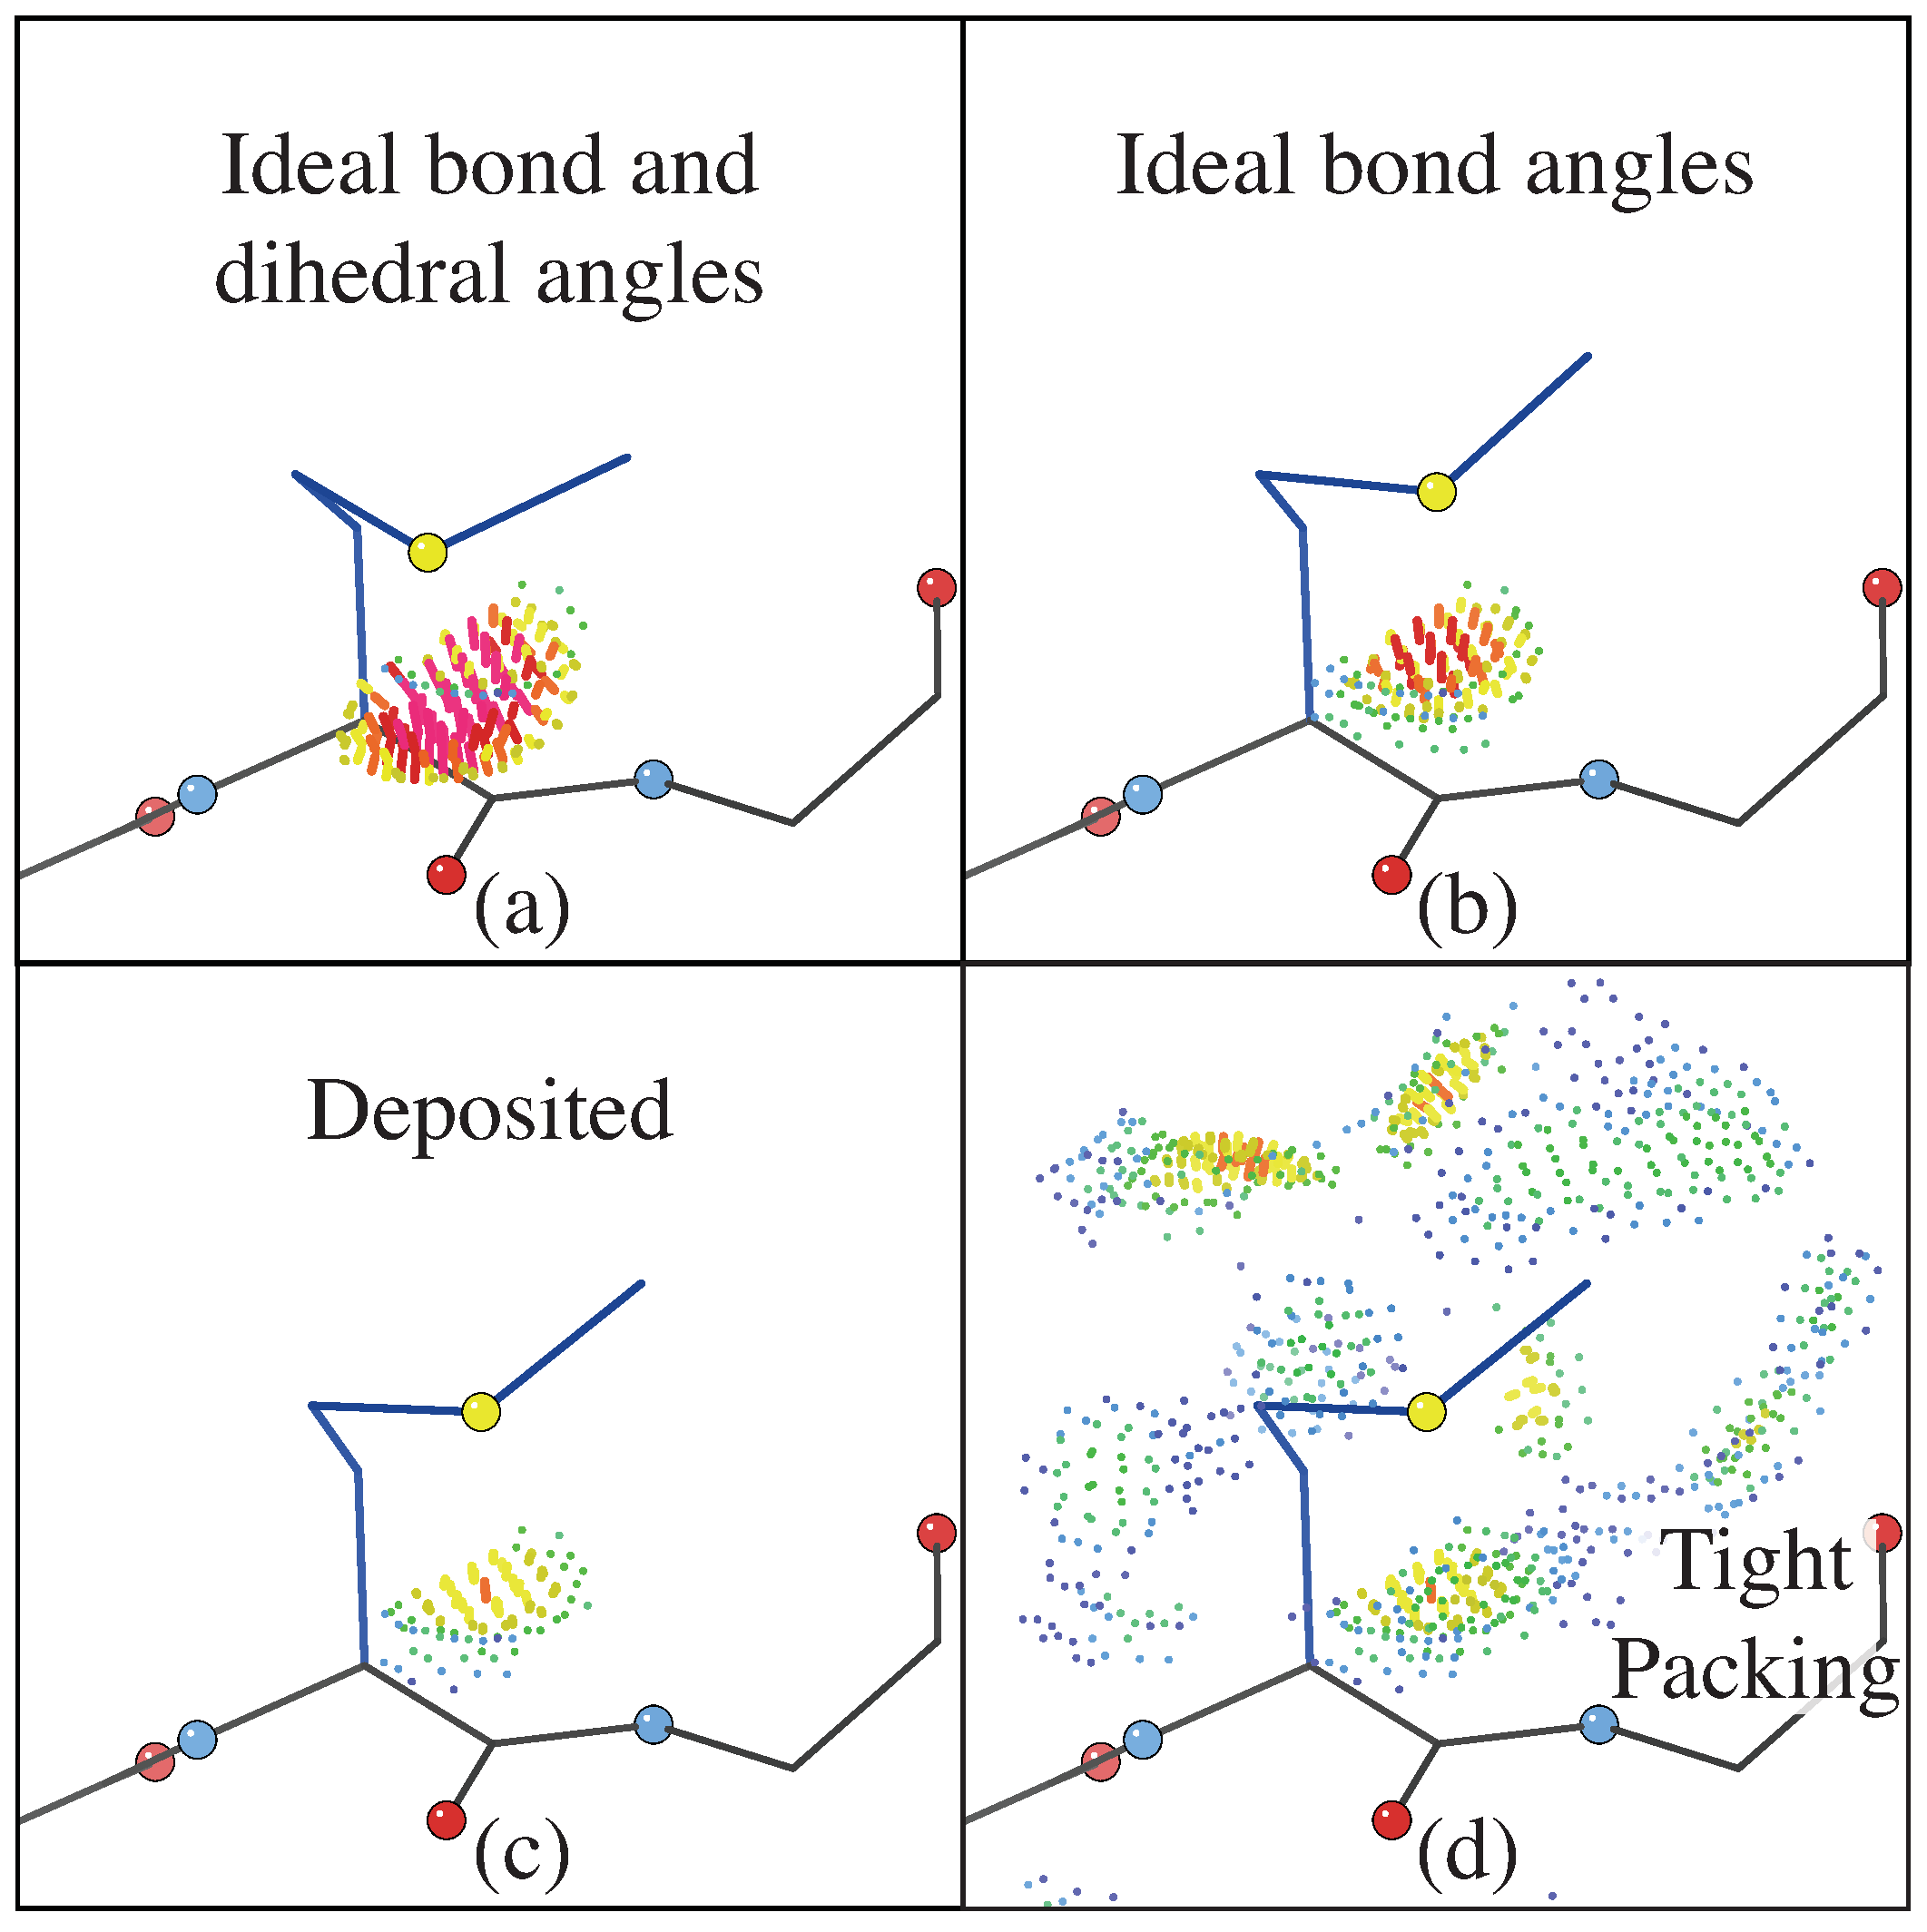
\includegraphics[width=0.5\textwidth]{MetPPP}
  \caption{\FigThreeCaption}
    \label{fig:2bmo}
\end{figure}



\begin{figure}[h]
  \centering
  \includegraphics[width=0.75\textwidth]{Glu_pm20_mp0}
\caption{\FigFourCaption}
\label{fig:Glupm20_mp0}
\vspace{-10pt}
\end{figure}


\begin{figure}[h]
  \centering
  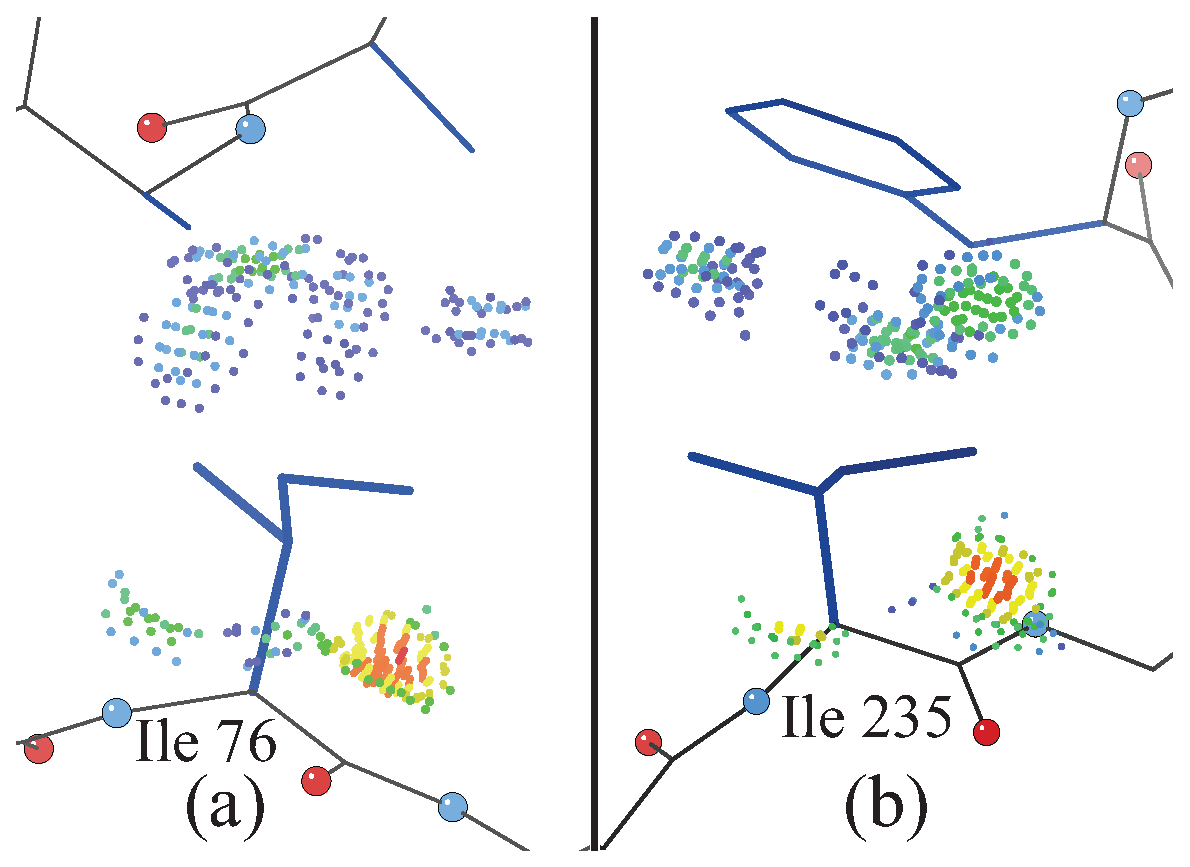
\includegraphics[width=0.5\textwidth]{IlePP}
\caption{\FigFiveCaption}
\label{fig:Ilepp}
\vspace{-10pt}
\end{figure}


\begin{figure}[h]
  \centering
  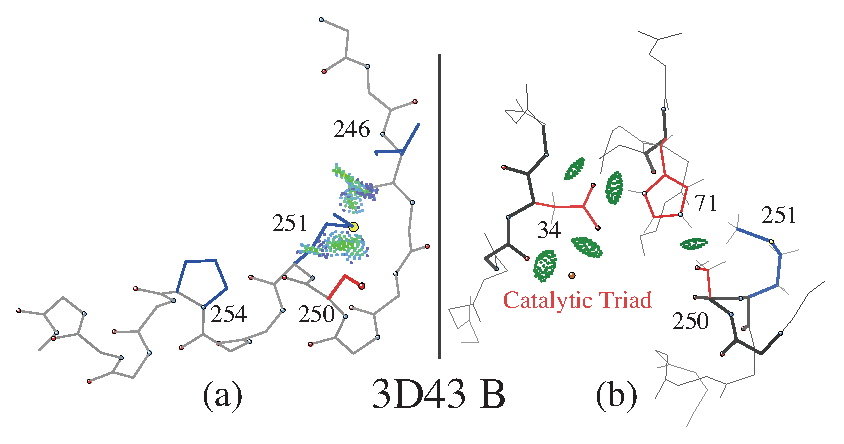
\includegraphics[width=0.95\textwidth]{Metmpm}
\caption{\FigSixCaption}
\label{fig:METmpm_3d43}
\vspace{-10pt}
\end{figure}


\begin{figure}[h]
  \centering
  \includegraphics[width=0.85\textwidth]{AspAsn_contours}
\caption{\FigSevenCaption}
\label{fig:AspAsn}
\vspace{-10pt}
\end{figure}



\begin{figure}[h]
  \centering
  \includegraphics[width=0.65\textwidth]{ASN_outliers}
\caption{\FigEightCaption}
\label{fig:AsnOutliers}
\vspace{-10pt}
\end{figure}


% acknowledgments
\clearpage
\section{Acknowledgments}
We would like to thank Richardson lab members Dan Keedy and Bryan Arendall for setting up the chain-level Top8000, Jeff Headd for moving the MolProbity utilities to use the \textit{PHENIX} cctbx toolbox, and Michael Prisant for help with GitHub. Also, thanks to \textit{PHENIX} Project members Nigel Moriarty and Nat Echols for help with integration into \textit{PHENIX} automation and GUI. This work was supported by NIH grants R01-GM073919 and ProjectIV of P01-GM063210, and by an NSF Graduate Research Fellowship to BJH.


\end{document}
